\documentclass[conference]{IEEEtran}
\IEEEoverridecommandlockouts
% The preceding line is only needed to identify funding in the first footnote. If that is unneeded, please comment it out.
\usepackage{cite}
\usepackage{amsmath,amssymb,amsfonts}
\usepackage{algorithmic}
\usepackage{graphicx}
\usepackage{textcomp}
\usepackage{tabularx,booktabs}
\usepackage{xcolor}
\usepackage[hidelinks]{hyperref}
\usepackage{subcaption}
\def\BibTeX{{\rm B\kern-.05em{\sc i\kern-.025em b}\kern-.08em
    T\kern-.1667em\lower.7ex\hbox{E}\kern-.125emX}}
\begin{document}

\makeatletter
\newcommand{\linebreakand}{%
  \end{@IEEEauthorhalign}
  \hfill\mbox{}\par
  \mbox{}\hfill\begin{@IEEEauthorhalign}
}
\makeatother

\title{The Power of Augmentation: Comparing Performances of StyleGAN Architectures}

\author{

\IEEEauthorblockN{Matej Ciglenečki}
\IEEEauthorblockA{\textit{Faculty of Electrical Engineering and Computing}\\
Zagreb, Croatia\\
matej.ciglenecki@fer.hr}


\and

\IEEEauthorblockN{Fran Čutura}
\IEEEauthorblockA{\textit{Faculty of Electrical Engineering and Computing}\\
Zagreb, Croatia \\
fran.cutura@fer.hr}

\linebreakand 

\IEEEauthorblockN{Dominik Matić}
\IEEEauthorblockA{\textit{Faculty of Electrical Engineering and Computing}\\
Zagreb, Croatia \\
dominik.matic@fer.hr}

\and

\IEEEauthorblockN{Filip Mirković}
\IEEEauthorblockA{\textit{Faculty of Electrical Engineering and Computing}\\
Zagreb, Croatia\\
 fm0035208855@fer.hr}

\linebreakand 

\IEEEauthorblockN{Ivan Rep}
\IEEEauthorblockA{\textit{Faculty of Electrical Engineering and Computing}\\
Zagreb, Croatia\\
ivan.rep2@fer.hr}

\and

\IEEEauthorblockN{Jakov Rukavina}
\IEEEauthorblockA{\textit{Faculty of Electrical Engineering and Computing}\\
Zagreb, Croatia\\
jakov.rukavina@fer.hr}
}

\maketitle

\begin{abstract}
Image generation is the task of generating new images from an existing dataset. With the advancement of graphics processing units, there has been a growing interest in this task. However, not everyone has the resources to train large models such as StyleGAN. In this paper, we discuss at which point bigger StyleGAN models overperform the StyleGAN2-ADA model on the MetFaces dataset. For comparison, we also use a deep convolutional generative adversarial network as a baseline and compare the results.
\end{abstract}

\begin{IEEEkeywords}
generative adversarial network, image generation, style transfer
\end{IEEEkeywords}

\section{Introduction}

A generative model tries to approximate a probability distribution $p(\mathbf{x})$ given a training set of examples. Besides generating new examples, this approach can be used for other tasks such as classification or anomaly detection. The difference between these models and discriminative models is that discriminative models approximate a different probability distribution, $p(y|\mathbf{x})$. Generating new samples is a harder problem than classifying existing ones. There are a lot of approaches for this task such as variational autoencoders, restricted Boltzmann machines, normalizing flows, or generative adversarial networks. The last technique has recently seen a lot of attention because of the rise of GPU computing and its effectiveness. This method uses two different models, a generator and a discriminator. The job of the discriminator is to classify an image into two classes: one for real images and one for fake images, while the generator tries to fool the discriminator by generating new convincing examples.
In this paper, we analyze different approaches such as deep convolutional generative adversarial networks. This is an extension of generative adversarial networks which uses convolutional and convolutional-transpose layers in the discriminator and generator. We also explore StyleGANs, which were introduced in $2018$ by Nvidia researchers. Our goal is to try to understand when it is better to train a StyleGAN2-ADA model instead of a StyleGAN2 model while keeping in mind the training time. Besides this, we explore and analyze the latent space vectors. The rest of this paper is organized as follows. Section 2. presents related work on image generation. In Section 3. we describe the datasets we use and the datasets that are most often used for this task. Section 4. explains the differences between each of the used architectures and Section 5. explains our experiments regarding DCGAN and StyleGAN. In Section 6. we discuss the results and in Section 7. we analyze the latent space and its properties. Finally, in Section 8. we present our conclusions.

\begin{figure}
	\begin{center}
		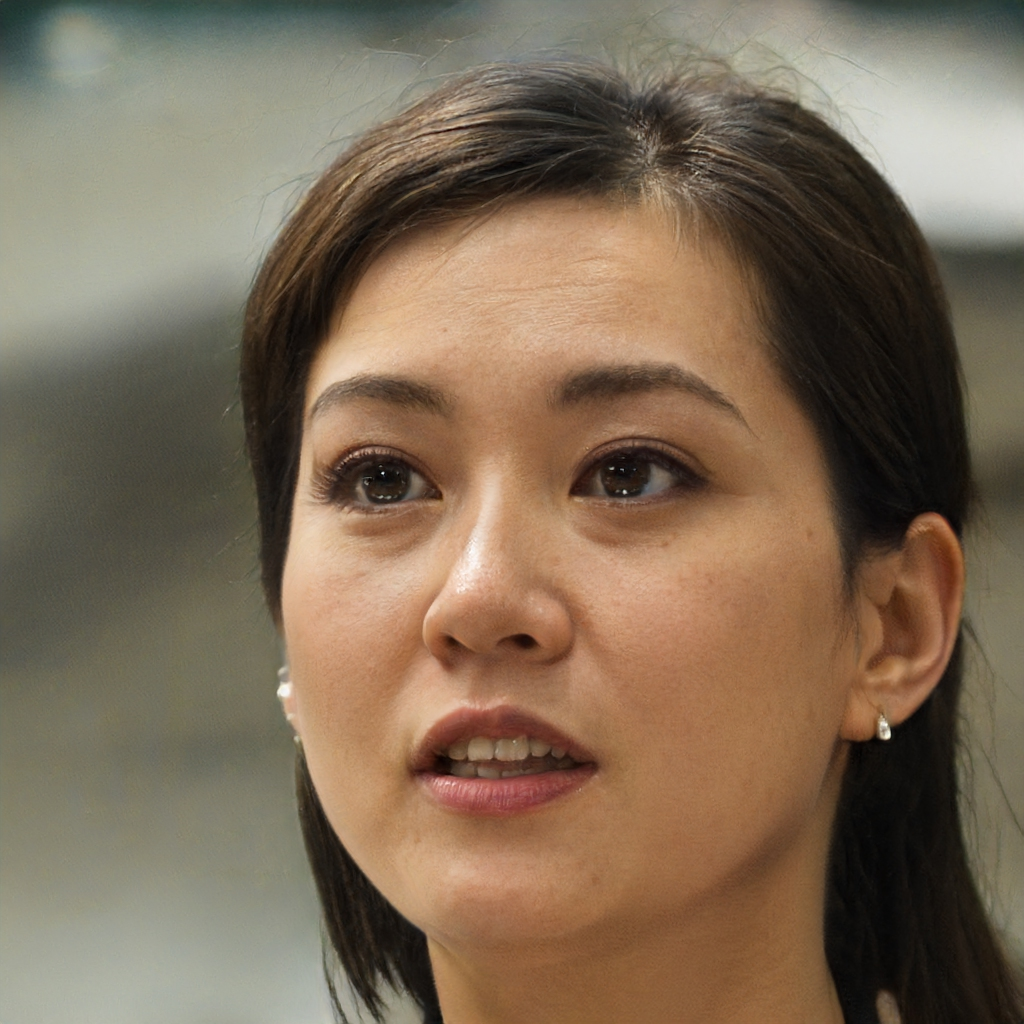
\includegraphics[width=0.48\columnwidth]{./images/doesntexist.jpg}
		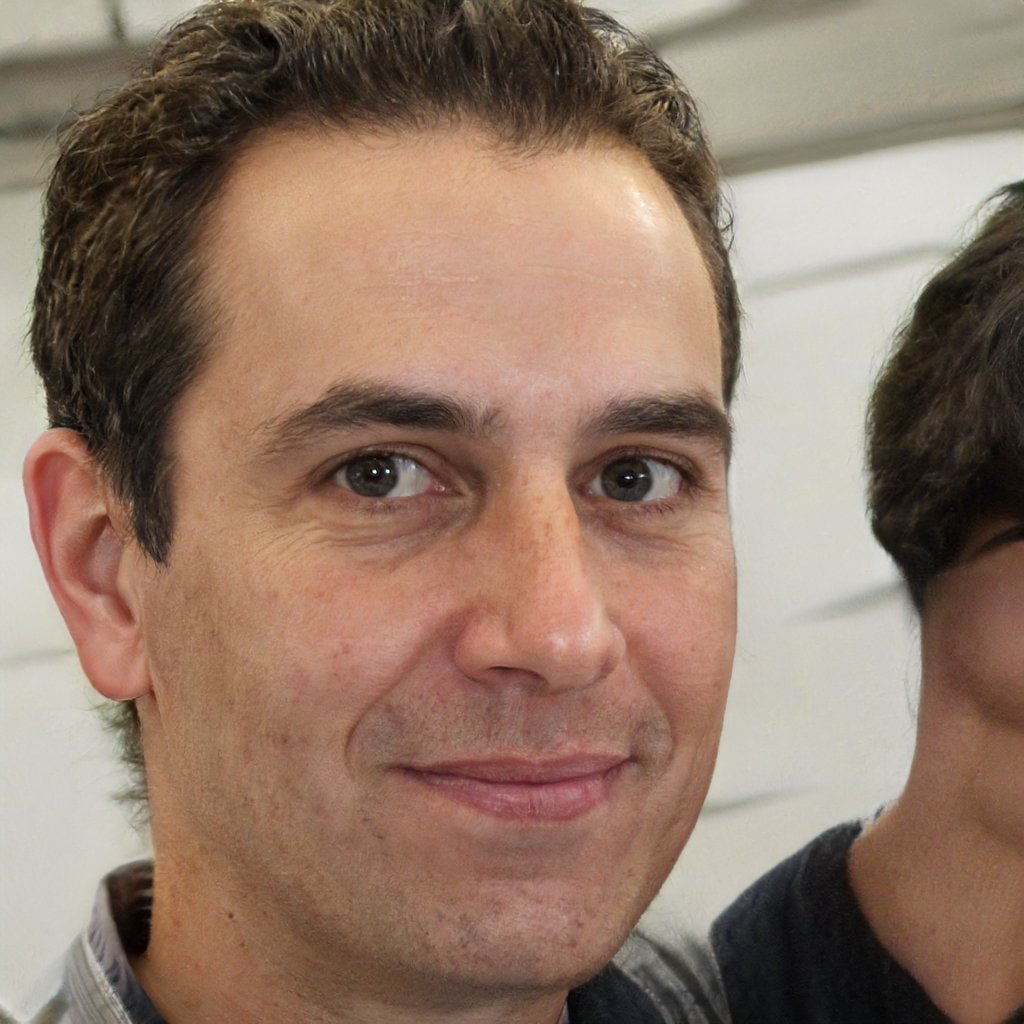
\includegraphics[width=0.48\columnwidth]{./images/doesntexist2.jpg}
		\caption{Examples of two images taken from \url{https://thispersondoesnotexist.com/}, which generates face images using a StyleGAN2 model.}
		\label{fig:figure1}
	\end{center}
\end{figure}

\section{Related Work}

In the past few years, more attention has been given to image generation. In 2016, researchers from Indico and Facebook \cite{DCGAN} proposed learning unsupervised representations using convolutional neural networks and introduced a new subclass called deep convolutional generative adversarial networks. These networks learn a hierarchy of representations from objects to whole scenes. Soon after, Nvidia researchers proposed an alternative generator architecture for generative adversarial networks \cite{STYLEGAN}. This architecture automates learning unsupervised representations of high-level attributes such as pose and low-level attributes such as hair. In its time, this model achieved state-of-the-art results using traditional quality metrics. Besides this, it demonstrated better latent representation properties, such as smoother interpolation. A year later, an improvement of StyleGAN was designed \cite{STYLEGAN2} which again yielded state-of-the-art results in unconditional image generation. This paper featured redesigning the generator normalization, discussing progressive growth and regularization of the generator to improve image quality. The problem with most of these previously mentioned papers was a large amount of computing power and large amounts of available data. StyleGAN2-ADA \cite{STYLEGAN2ADA} addresses this problem by proposing an adaptive discriminator augmentation mechanism that stabilizes training with limited amounts of data. An important detail is that this technique applies to previously designed models and requires no changes to loss functions or network architectures. This method requires only a few thousand training images. Finally, the last improvement are Alias-Free Generative Adversarial Networks \cite{STYLEGAN3} which discuss coupled details and image coordinates. A solution for this problem is small architectural changes that match the quality metrics of StyleGAN2 but differ in their internal representations.

\section{Data}
There are many benchmark datasets for the image generation task. Some of these are BreCaHAD, a dataset for breast cancer and histopathological annotation, AFHQ, a dataset of high-quality images of animal faces, CIFAR-$10$, which contains tiny images of $10$ classes, FFHQ, a dataset of high-quality images of human faces and MetFaces, a dataset of human faces extracted from works of art. The StyleGAN papers train models for each of these datasets at different resolutions.

The FFHQ dataset consists of $70 000$ aligned and cropped images at $1024 \times 1024$ resolution. These images were crawled from Flickr and contained a lot of diversity, covering different ages, ethnicities, and image backgrounds.
The MetFaces dataset contains $1336$ high-quality PNG images at $1024 \times 1024$ resolution and was crawled using The Metropolitan Museum of Art Collection API, aligned and cropped.
The CelebA dataset contains $202 599$ images of celebrities with a lot of diversity and rich annotations. There is also a version of the dataset with aligned and cropped faces.

\begin{figure}[!h]
	\begin{center}
		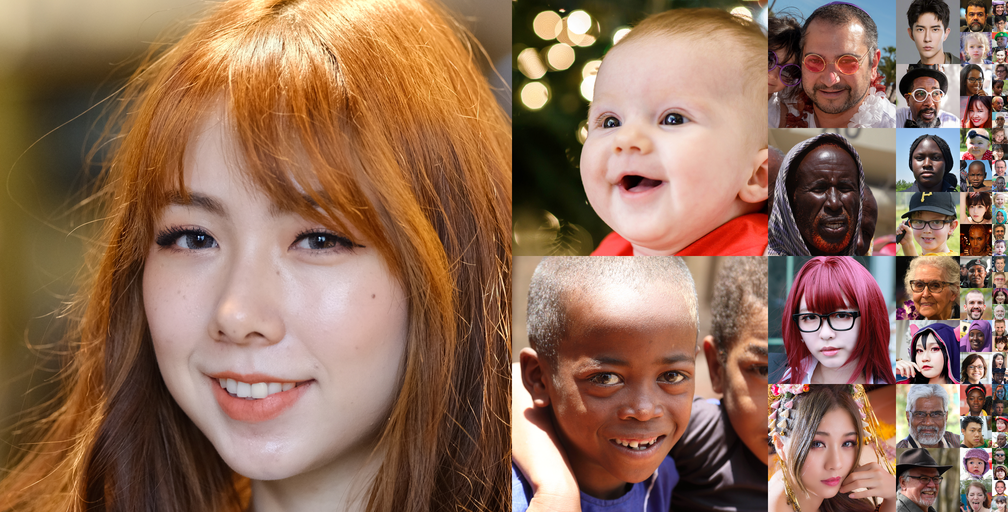
\includegraphics[width=1\columnwidth]{./images/ffhq-teaser.png}
		\caption{Examples of images taken from the FFHQ dataset.}
		\label{fig:figure2}
	\end{center}
\end{figure}

\begin{figure}[!h]
	\begin{center}
		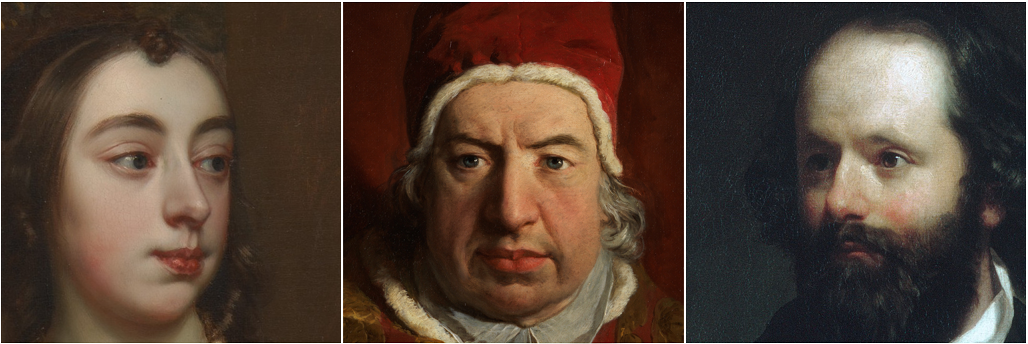
\includegraphics[width=1\columnwidth]{./images/metfaces-teaser.png}
		\caption{Examples of images taken from the MetFaces dataset.}
		\label{fig:figure3}
	\end{center}
\end{figure}

\section{From GAN to StyleGAN}

The original GAN generator is fed a latent vector $\mathbf{z} \in \mathbb{R}^l$ which is progressively upscaled through the network to produce images of a certain resolution. A typical setup is the well-known DCGAN, which uses convolutional layers with a stride greater than unity (usually $2$) to upscale the image. There are plenty of issues that arise with the images produced with such GANs most commonly there are visible model artifacts in the generated images and there is virtually no interpretability of the latent space i.e. it is not clear which components contribute to which attributes of the images. The Style GAN architecture provides remedies to this.
Many new parts make up the StyleGAN generator, the most obvious one is the way latent vectors are fed to the network. Contrary to most GAN architectures the first layer of the StyleGAN is not some latent vector or a convolutional/linear layer waiting to be fed the said vector, rather it is a learnable constant tensor, that tensor usually has the shape $C \times 4 \times 4$. The shape of the tensor indicates that it may be treated as a $C$-dimensional $4 \times 4$ image, which is progressively upscaled to the final desired resolution.
Where then does the latent vector come into play? The latent vector $\mathbf{z}$ is first passed through a smaller fully connected neural network to produce a style vector $\mathbf{w}$. This vector enters the generator at various points via the adaptive instance normalization, which will be discussed in greater detail in the following subsection.

\begin{figure}[!h]
	\begin{center}
		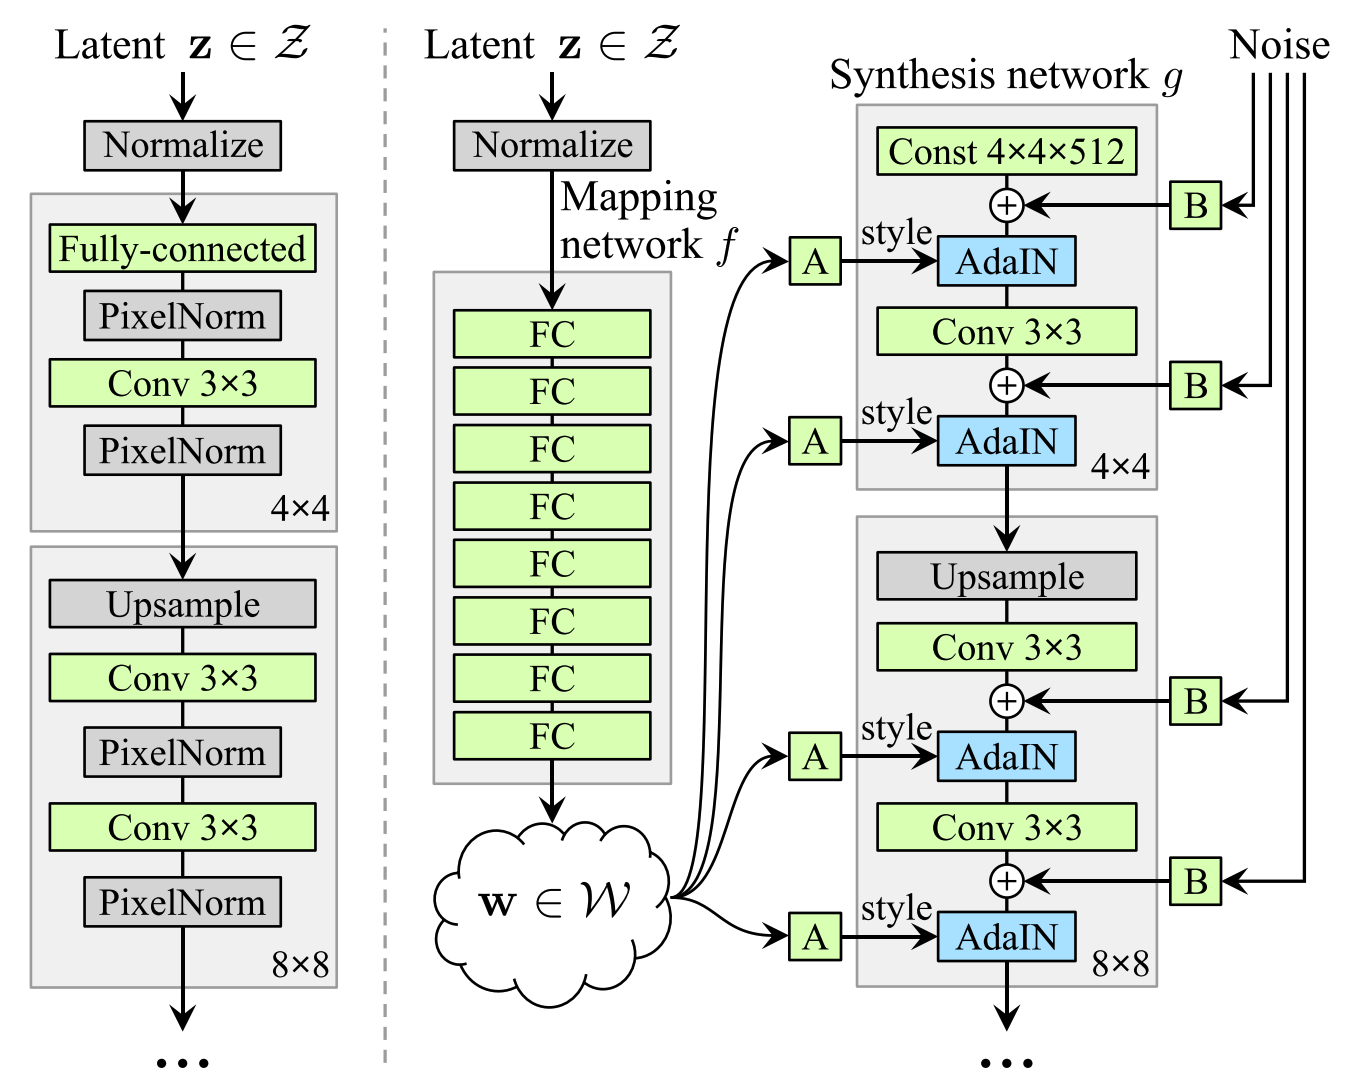
\includegraphics[width=1\columnwidth]{./images/stylegan.png}
		\caption{Comparison of the traditional generator (left) and the StyleGAN generator(right).}
		\label{fig:figure4}
	\end{center}
\end{figure}

	Another novelty is the addition of gaussian noise after every convolution operation. To be more concrete a tensor containing gaussian noise is created, its shape is $1 \times H \times W$ where $H$ and $W$ are the height and width of the image produced in a certain layer. To pass this noise to all channels the network introduces yet another learnable tensor $B$ shaped $C \times 1 \times 1$, it then multiplies the noise tensor which is added to the layer output. We can think of tensor $B$ as the tuning per channel noise. If this noise is present only in the low-resolution layers it controls coarse features such as the shape of the face or beard and no beard, however, at high resolutions, it controls some of the facial features that are usually stochastic such as beard and hair placement or freckles. The addition of this noise can greatly add to the realisticity of the generated images.
Lastly, as shown in the figure \ref{fig:figure4}, higher resolutions are obtained by bilinear upsampling, this allows for the so-called progressive training. After every block, we are left with an image of some resolution we can train the generator-discriminator pair progressively i.e. first train them on lower resolutions and add layer by layer to increase the image complexity. This has become one of the staple procedures for training GANs that deal with high-resolution images, and it is not just a feature of the StyleGAN.



\subsection{Adaptive instance normalization in StyleGANs}
The simple batch normalization's success in training neural networks led to more extensive experimentation of the various possible normalizations and their usefulness, thus yielding adaptive instance normalization (ADAIN). We find the explanation provided in \cite{ADAIN} to our liking and follow the author's explanation in this paper as well.
The path to ADAIN is made in three steps. Consider the action of the familiar batch normalization (BN).

\begin{equation}
	\label{eq:1}
	BN(x) = \gamma \frac{x -  \mu(x)}{\sigma(x)} + \beta
\end{equation}

Here the $x$ is the tensor $x \in \mathbb{R}^{NxCxHxW}$ where $N$ is the batch size and $\gamma$,  $\beta \in \mathbb{R}^C$. Consequently the mean and standard deviation are calculated across the batch for each channel (feature), for instance:

\begin{equation}
	\mu(x)_c = \frac{1}{NHW}\sum_{nhw}x_{nchw} 
\end{equation}

In tasks such as style transfer, a useful shift from BN has been to the so-called instance normalization (IN), here means and standard deviation are calculated across the height and width dimensions i.e. every instance in the batch and every channel of that instance get normalized

\begin{equation}
	\mu(x)_{nc} = \frac{1}{HW}\sum_{hw}x_{nchw} 
\end{equation}

And the normalization itself is analogous to the one present in the equation (\ref{eq:1}). 
The reasons for the success of IN were not completely clear from a theoretical standpoint, however, it prompted further investigation in the same direction leading to ADAIN.

The idea is simply to add another vector $w$ which can control the normalization parameters in some way. Or we can interpret this in a way that the normalization is being learned, whichever standpoint we take the procedure is the same. The vector $w$ we obtained from the mapping network is passed through a learnable linear layer to output the vector $y \in \mathbb{R}^{2C}$. This vector is further split into two $C$-dimensional vectors that are interpreted as the adaptive mean and standard deviation.

\begin{equation}
	ADAIN(x,w) = y_s(w)\big(\frac{x - \mu(x)}{\sigma(x)} 	\big) +  y_m(w)
\end{equation}

The mean and standard deviation are calculated in the same way as in the IN case. This is how styles enter the generator network.





\subsection{Adaptive Discriminator Augmentation}
The persistent problem with training deep neural networks is the need for large datasets. This problem is even more exaggerated in GANs. What usually happens is that to train a powerful generator an even more powerful discriminator is needed, the pitfall of overly complex models is that they can memorize every instance of the training dataset if this happens the discriminator no longer provides useful input to the generator.
A standard remedy for lack of data is its augmentation, however, if we augment the images in the dataset the generator will learn to create augmented images which is an undesirable result. What the authors of \cite{STLEGAN2ADA} propose is a certain augmentation pipeline. Assume we have a total of $M$ transformations which we intend to use to augment our data. We will not perform those transformations directly on the dataset rather we will perform the transformations on the images right before they enter the discriminator, also we perform every transformation with a certain probability $p$. This is done for the images from the training set and the ones generated by the generator.
If the number M is large and $p$ above $0.5$ the chance that the discriminator sees an unaugmented image is very low i.e. it rarely sees the original images. This leads to the seemingly larger dataset and the augmentations do not lead to the generator. The only requirement is that the augmentations are differentiable so a proper backpropagation can be performed. Supposedly this improves the convergence of the algorithm and the resulting image quality.
What remains to be determined is the value of the probability $p$, it’s not likely that one fixed value will suffice throughout the entire training. Here is where the adaptive comes from in the subsection title. In \cite{STYLEGAN2ADA} the authors propose tuning parameters that track the discriminator overfitting and therefore the probability $p$. For both the intuition is the same we do not want to let $\mathbb{E}(D_{training}$ become too close to one. Where $D_{training}$ is the discriminator output on the training set.

\begin{equation}
	r_v = \frac{\mathbb{E}(D_{train}) -\mathbb{E}(D_{valid})}{\mathbb{E}(D_{train}) -\mathbb{E}(D_{generated})}
\end{equation}

\begin{equation}
	r_t = \mathbb{E}(sign(D_{train}))
\end{equation}

$p$ is initially set to $0$ and after every $4$ minibatches these overfitting heuristics are calculated if they indicate overfitting $p$ is increased by a fixed amount, if there is underfitting $p$ is decreased by the same amount.


\section{Experimental setup}

\subsection{StyleGAN2 vs. StyleGAN2-ADA}
In this section, we compare the results of the original StyleGAN2 to the StyleGAN2-ADA (StyleGAN2 which uses Adaptive Discriminator Augmentation). Instead of starting from scratch, the starting point of this experiment is a pretrained StyleGAN2 trained on the FFHQ $256 \times 256$ resolution dataset. Using this model, four different training sessions were run consequently. The differences between the training sessions are the use of ADA (Adaptive Discriminator Augmentation vs. no augmentation) and the dataset size (dataset vs. subset of the dataset). Models are fine-tuned on the MetFaces, a $1336$ high-quality image dataset of human faces extracted from works of art. This particular dataset is a great candidate for fine-tuning a pretrained StyleGAN2 trained on the FFHQ since the domain gap between FFHQ’s images (photos of faces) and MetFaces’ images (artworks containing faces) isn’t huge. Every hyperparameter defaults to the "paper256" config of StyleGAN2-ADA project unless said otherwise. The total number of kimg is $100$ for all experiments (kimg represents the number of thousands of images that passed through the model during the training). The initial sample of the FFHQ dataset is presented. Results for each training session will be shown for the sample

\begin{figure}[!h]
	\begin{center}
		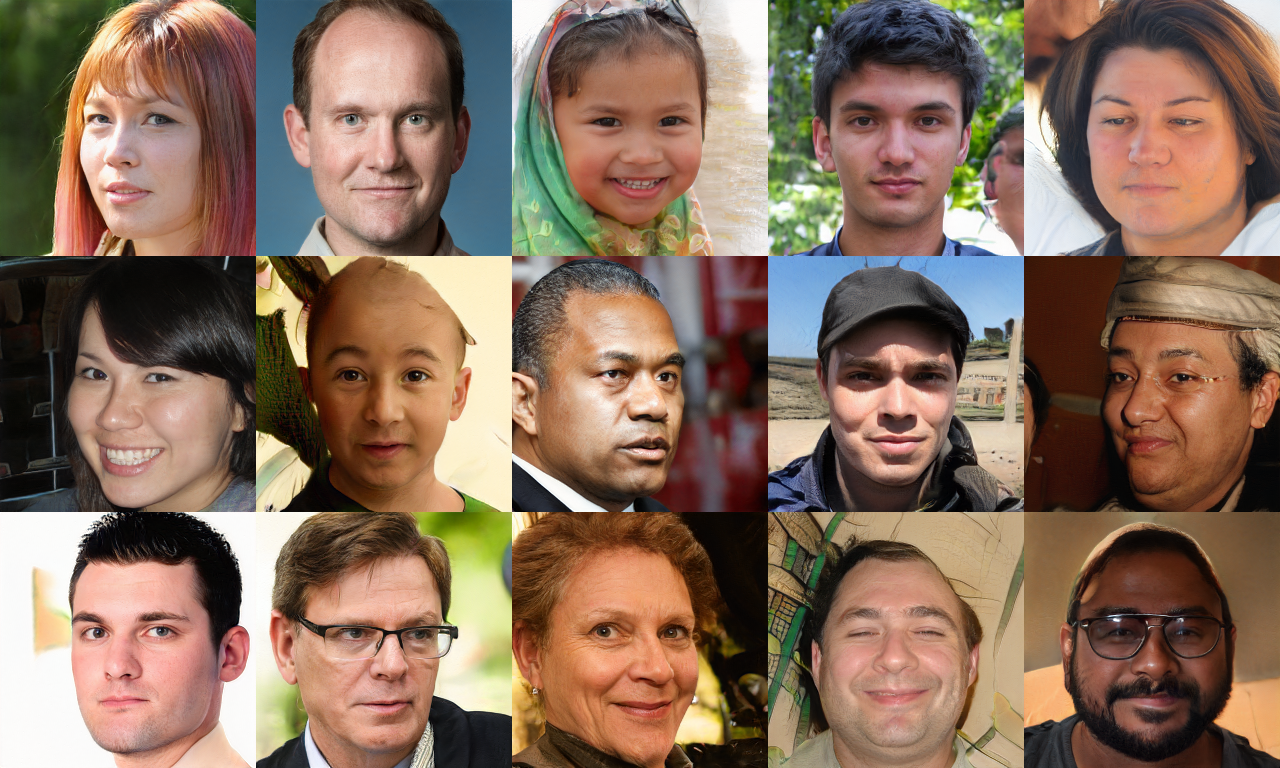
\includegraphics[width=1\columnwidth]{./images/picked_images/stylegan2_beginning.png}
		\caption{Random sample generated with StyleGAN2 pretrained on FFHQ dataset.}
		\label{fig:figure5}
	\end{center}
\end{figure}
%(stylegan2_beginning.png)[Random sample generated with StyleGAN2 pretrained on FFHQ dataset]

First, StyleGAN2 and StyleGAN2-ADA are compared after being fine-tuned on the whole MetFaces dataset (1336 images). Both StyleGAN2 and StyleGAN2-ADA produce similar results after the same amount of kimg steps. StyleGAN2-ADA preserves the facial structure and features slightly better, while the StyleGAN2 sacrifices facial similarity to the original face to generate an image that looks more like an artwork than a photo. For this experiment, the advantage of using ADA is not obvious nor necessary.

\begin{figure}[!h]
	\begin{center}
		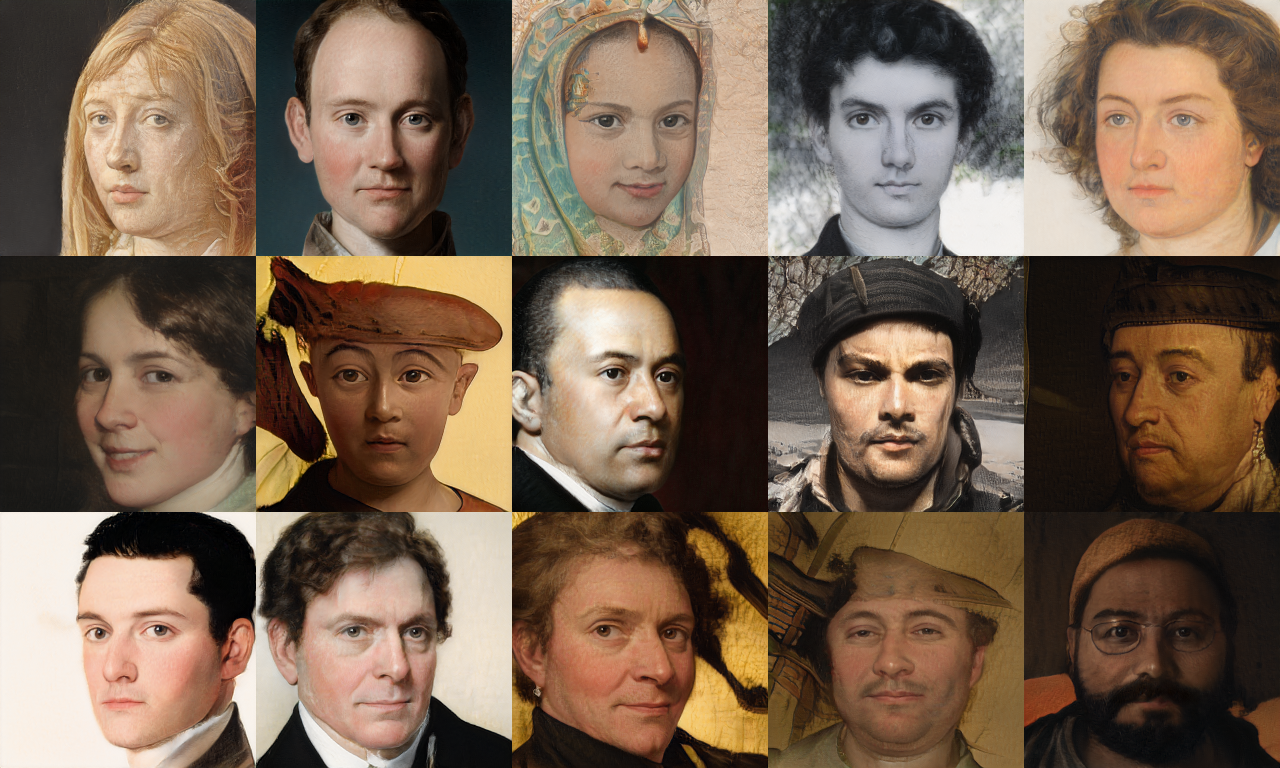
\includegraphics[width=1\columnwidth]{./images/picked_images/stylegan2_ADA_step_40_full_dataset.png}
		\caption{kimg 40 step of the StyleGAN2-ADA model fine-tuned on the whole MetFaces dataset.}
		\label{fig:figure6}
	\end{center}
\end{figure}
%(stylegan2_ADA_step_40_full_dataset.png)[kimg 40 step of the StyleGAN2-ADA model finetuned to the full MetFaces dataset]

\begin{figure}[!h]
	\begin{center}
		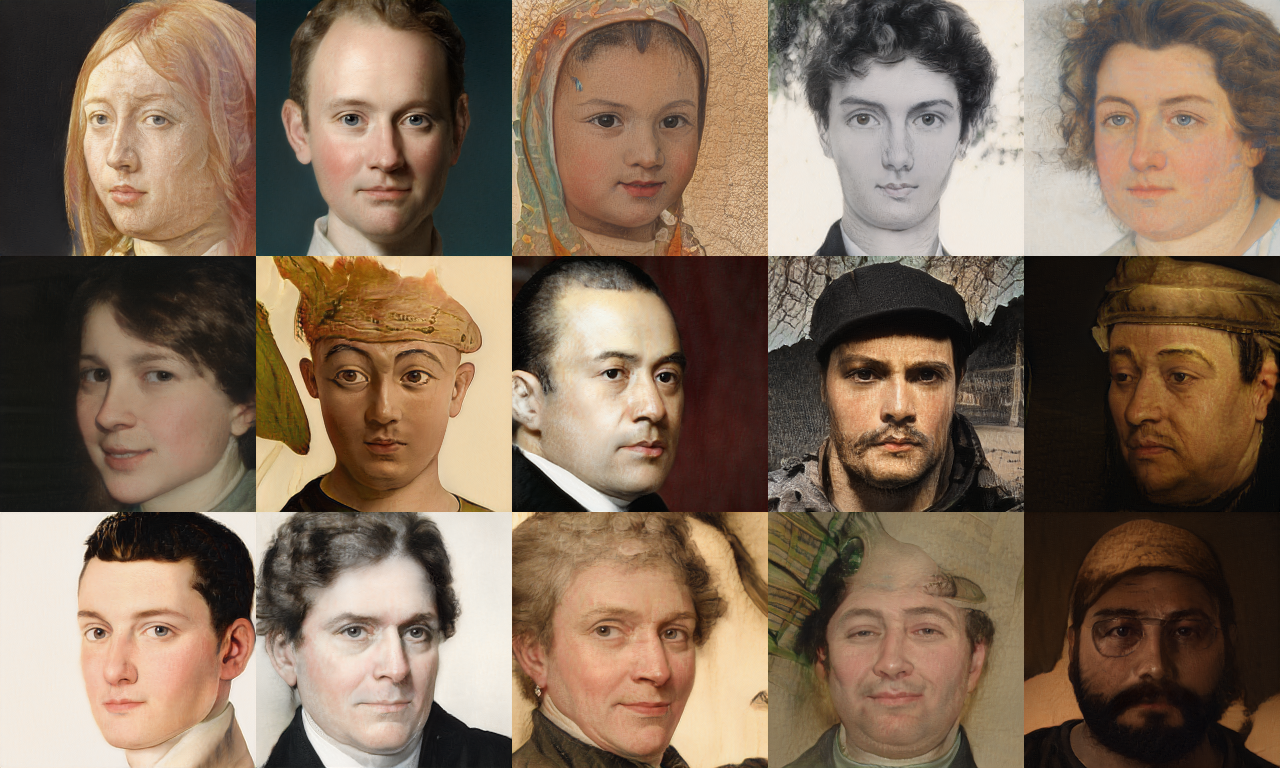
\includegraphics[width=1\columnwidth]{./images/picked_images/stylegan2_step_40_full_dataset.png}
		\caption{kimg 40 step of the StyleGAN2 model fine-tuned on the whole MetFaces dataset.}
		\label{fig:figure7}
	\end{center}
\end{figure}
%(stylegan2_step_40_full_dataset.png)[kimg 40 step of the StyleGAN2 model finetuned to the full MetFaces dataset]

Second, StyleGAN2 and StyleGAN2-ADA are compared after being fine-tuned on the subset of the MetFaces dataset ($100$ images). Both models in both training sessions received the same subset of $100$ images. Here, the advantage of using ADA is a tad more obvious. It seems that ADA augmentation preserves the facial structure (pose, smiles, face width…) better than the model which doesn’t use any augmentations. For kimg = $40$ it’s obvious that the model which didn’t use augmentation overfitted to a particular instance from the dataset while ADA generates a face that compromises between art and the original face. Rather than relying solely on subjective conclusions, the Fréchet inception distance (FID) [7] was calculated for both models. The FID metric is similar for both models at the start, but StyleGAN2-ADA’s performance overtakes at kimg = $30$ because the StyleGAN2 starts overfitting to the small dataset.

\begin{figure}[!h]
	\begin{center}
		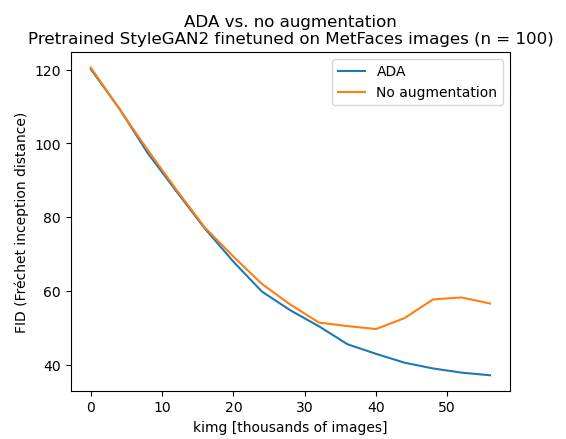
\includegraphics[width=1\columnwidth]{./images/fid_ada_vs_noada.png}
		\caption{FID metric of StyleGAN2 and StyleGAN2-ADA fine-tuned on MetFaces images (n = 100).}
		\label{fig:figure8}
	\end{center}
\end{figure}
%(fid_ada_vs_noada.png)[FID metric of StyleGAN2 and StyleGAN2-ADA finetuned on MetFaces images (n = 100)]

\subsection{MiniStyleGAN}
Most of the problems with experimenting and tweaking the StyleGAN2-ADA network arise from the sheer size of the model. Meaning that any slight change or attempt at fine-tuning will inevitably end in training the model again. In absence of sufficient hardware that training can prove to be an insurmountable challenge, this motivated us to explore the effectiveness of the StyleGAN at lower resolutions. We experimented with a range of models that implement various aspects of the full StyleGAN on low-resolution images ($64 \times 64$). We dub these models miniStyleGANs even though some can be very dissimilar from the original.
The images for training were drawn from the CelebA dataset and rescaled to the desired resolution with bicubic interpolation.
The models in question are the following:
\begin{enumerate}
	\item A smaller StyleGAN generator \cite{STYLEGAN} with bilinear upsampling
	\item A DCGAN that feeds the latent vector multiple times - once in the standard DCGAN fashion, otherwise the vector $\mathbf{z}$ is passed through the mapping network to get the style vector $\mathbf{w}$ which enters the generator again through adaptive instance normalization
	\item The last model considered was a proper StyleGAN that uses transposed convolutional layers for upsampling. This model starts with a learnable constant tensor much like the original StyleGAN.
\end{enumerate}

For all three generators a simple DC discriminator was used, this choice for this was mostly due to the computational requirements of the generators being high thus a simpler discriminator was necessary. The authors still find this advantageous since the performance of the three generators can be compared with a non-variable discriminator.

\subsection{Training setup and network specifics}
All three generators possessed the same latent space dimensionality of $128$ which is significantly lower than the original $512$, these cuts were made with computational efficiency in mind. The batch size for training was $128$ except for the pure styleGAN which had to be trained with mini-batches of $64$ images, due to hardware constraints. The training regime was also a hyperparameter, it consists of two integers representing the number of steps the discriminator makes while training followed by the number of steps the generator makes; this was typically set to $(5, 3)$ or $(4, 3)$. Instead of the number of epochs, we specify the total number of steps these networks will do. This was set to 8000, again except for the pure styleGAN which required longer training for satisfactory results. The styleGAN was trained for $16000$ steps. This meant that the first two networks trained in $4$ hours while the last one required $9$ hours.
The optimizer for each generator and discriminator was always Adam with the same learning parameters: learning rate was $0.0001$, and $(\beta_1,\beta_2) = (0, 0.99)$. Lastly, the training was performed using an Nvidia GeForce GTX $1650$ Mobile / Max-Q GPU.

\section{Results}

\subsection{Mini StyleGAN}
Upon first glance, all three models generate similar images, albeit styleGAN architectures exhibit a higher degree of mode collapse. However, one of the challenges with GANs is quantifying the quality or realism of the images they produce, using a human for that estimation is unacceptable.
To this end, deep neural models are employed to assess the quality of generated images. This is done by training a feature detection model $\mathcal{F}$, a feature is essentially a tensor of shape $(C_l,H_l,W_l) \, l = 1,...,L$. The \textit{similarity} or rather \textit{distance} between two images is defined as \cite{PERCSIM}.
\begin{equation}
d(x,x_0) = \sum_l \frac{1}{H_l W_l} \sum_{h,w}|| y_{hw}^l - y_{0hw}^l ||^2_2
\end{equation}
Here $y$ represents the calculated feature vectors. The lower the $d$ is the more similar the two inmates are, this metric has been shown to correlate highly with the human notion of similarity \cite{PERCSIM}.
We used the pretrained AlexNet model for similarity estimation. A $1000$ images were randomly sampled from the training set, furthermore, we generated another $1000$ images with each model and calculated the mean learned perceptual images similarity metric (LPIPS) for every model. This will in essence measure the similarity between the generated images and the training dataset, however, the hope is that the dataset is representative of realistic images. The results seem to validate the intuition, all three models had a very similar LPIPS metric, with the styleGAN with deconvolutional upsampling having the best results. The distances are presented in the table \ref{tab:results}, here lower metric means more realistic image generation.


\begin{table}[!h]
	\begin{center}
		\caption{LPIPS values using different models}
		\begin{tabular}{ll}
			\toprule
			Model & LPIPS \\
			\midrule
			Style with deconv & 0.358\\
			DCGAN & 0.367 \\
			StyleGAN & 0.374 \\
			\bottomrule
		\end{tabular}
		\label{tab:results}
	\end{center}
\end{table}
%TABLICA FID-ova…
%
%Slike negdje u Appendixu?


\section{Intermediate latent space properties}

Since GAN architectures usually use an input layer that transforms it into latent code, style-based generators differ from this by using a learned constant and instead use a latent code $\mathbf{z}$ as an input. The generator then uses a mapping network that maps the latent code $\mathbf{z}$ to an intermediate latent representation $\mathbf{w}$. An interesting way we can use this insight is by taking a latent code $\mathbf{z}_1$ that represents the first image and a second latent code $\mathbf{z}_2$ that represents the second image. Using the mapping network we can calculate their intermediate latent representation $\mathbf{w}_1$ and $\mathbf{w}_2$. This means we can interpolate between these two vectors. Finally, for each of the vectors created by interpolation, we can use the synthesis network $g$ which will give us a smooth and meaningful transition from the first image to the second image. The official implementation uses an $18 \times 512$ matrix, with $18$ identical row vectors, so interpolation is done on matrices instead.

We can extend a similar idea to arbitrary many images. We can generate intermediate latent representations $\mathbf{w}_1, \hdots, \mathbf{w}_n$ and use a weighted average of these vectors to get a new representation. By using the synthesis network $g$, this average can be transformed into a new face that contains a certain amount of each person in it.
\begin{figure}[!htbp]
\begin{center}
	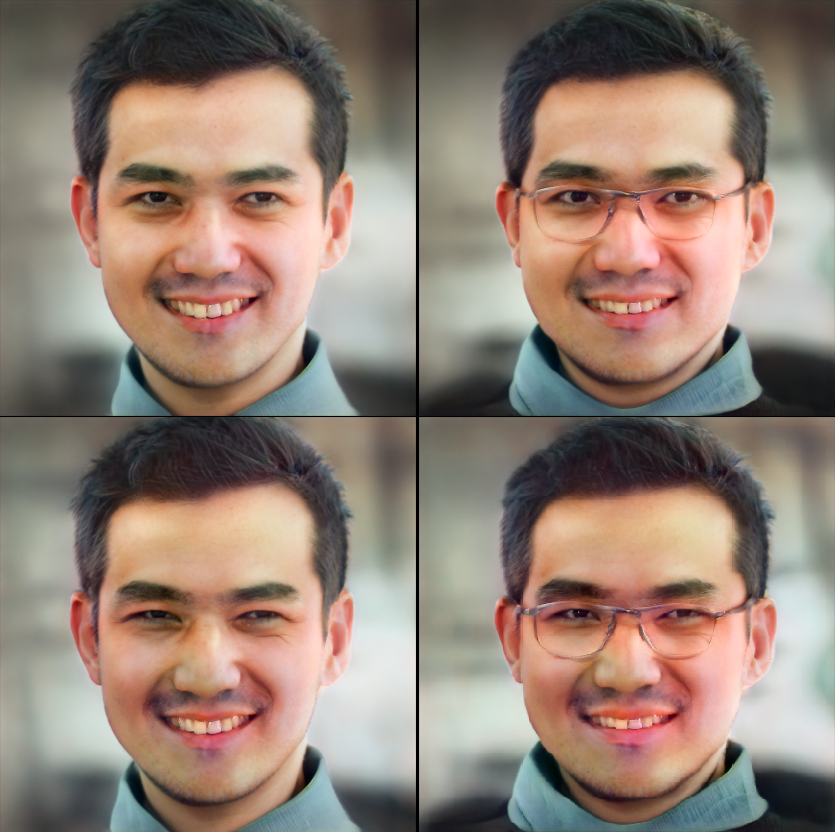
\includegraphics[width=1\columnwidth]{./images/w0-from-0-to-3.png}
	\caption{The figure shows the original image (upper left), the change of image when $3$ is added to the value of $\mathbf{w}_0$ (upper right), the change of image when $2$ is added to the value of $w_7$ (lower left) and the change of image when $2.5$ is added to both values (lower left). The feature controlled by $w_0$ adds glasses while the feature controlled by $\mathbf{w}_7$ determines how much the eyes are squinted.}
	\label{fig:figure9}
\end{center}
\end{figure}

Also, an interesting finding is that some of the features in the intermediate latent space correspond to meaningful real-life features. For example, feature zero decides whether the person has glasses, feature one shrinks the head of the person, feature three determines how elongated a face is, etc.

We further explore this by adding and subtracting constant values from row vectors $\mathbf{w}_i$ and $\mathbf{w}_j$ of our intermediate latent representations and we notice that the effect of these features truly is combined after using the synthesis network. For example, if we combine the effect of feature zero and feature seven the output is a person with glasses and squinted eyes. This also extends when combining more features, although the amplification of one feature affects other features.

We also wanted to determine which features affect which part of the face and how they affect it. The results are presented in the table \ref{tab:interpretations}. 
\begin{table}[!h]

		\caption{Interpretations for images after altering row vector values}
		\label{tab:interpretations}
		\begin{center}
			\begin{tabular}{ll}
				\toprule
				The row vector modified & Interpretation \\
				\midrule
				0 & glasses \\
				1 & cranium size\\
				2 & smile intensity\\
				3 & face length\\
				4 & teeth showing\\
				5 & lighting effect\\
				6 & eyebrow thickness, also affects facial hair\\
				7 & eye squint\\
				8 & eyebrow height, lighting effect on hair\\
				9 & eyebags\\
				10 & age, grey hair\\
				11 & circles under eyes, eyelash thickness, iris size\\
				5, 12 to 17 & lighting effect\\           
				\bottomrule
			\end{tabular}
		\end{center}
	\end{table}

\section{Conclusion}

In this paper we analyzed the significance of augmentation on transfer learning with limited data. We used StyleGAN2 and StyleGAN2-ADA compared to different subsets of the MetFaces dataset. Results suggest that in limited data surroundings, StyleGAN2-ADA outperforms the StyleGAN2 architecture. Besides this, we experiment with simplified GAN architectures by training from scratch and with intermediate latent space properties. In future work, we propose experimenting with transfer learning on different resolutions and altering only certain elements of the row vectors $\mathbf{w}$.


\bibliographystyle{ieeetran}
\bibliography{bibliography.bib}
\nocite{*}

\vspace{12pt}


\appendix

\begin{figure}[!h]
	\begin{center}
		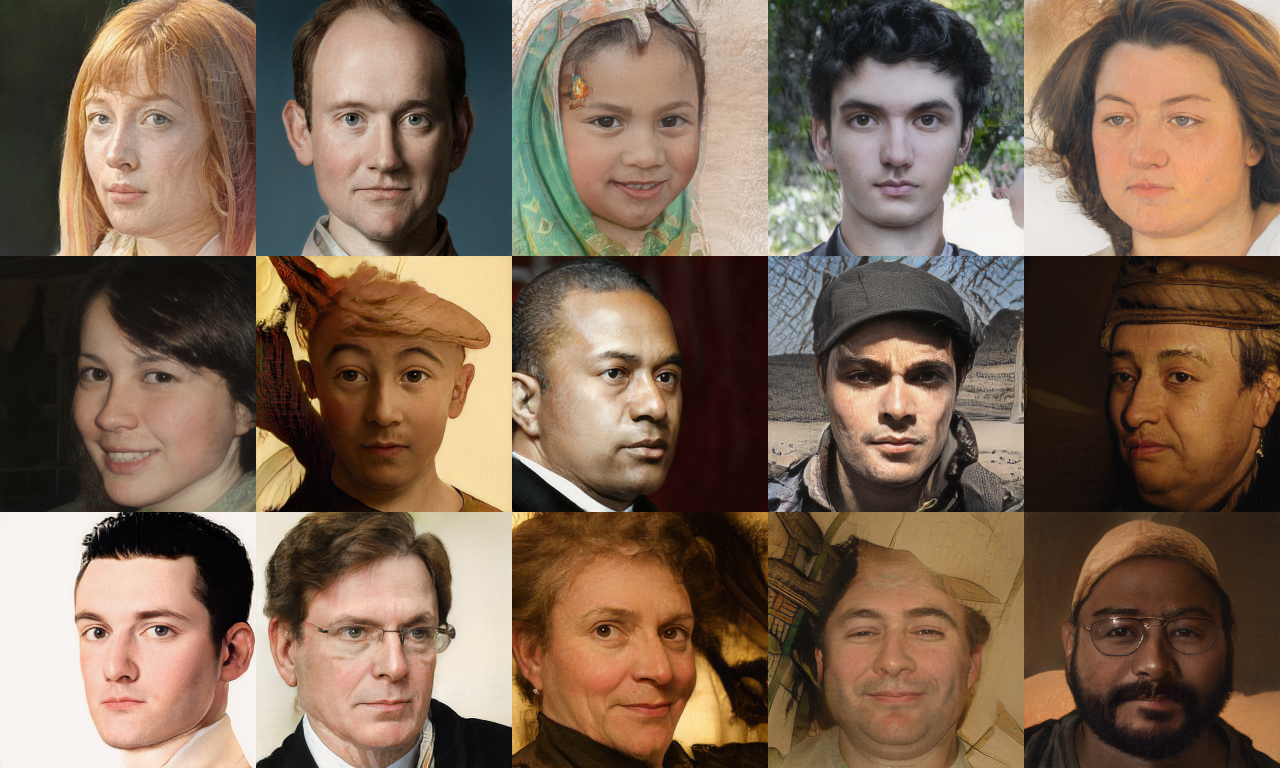
\includegraphics[width=0.8\columnwidth]{./images/picked_images/stylegan2_ADA_step_20_full_dataset.png}
		\caption{kimg 20 step of the StyleGAN2-ADA model fine-tuned on the whole MetFaces dataset.}
		\label{fig:figure10}
	\end{center}
\end{figure}
%(stylegan2_ADA_step_20_full_dataset.png)[kimg 20 step of the StyleGAN2-ADA model finetuned to the full MetFaces dataset]


\begin{figure}[!h]
	\begin{center}
		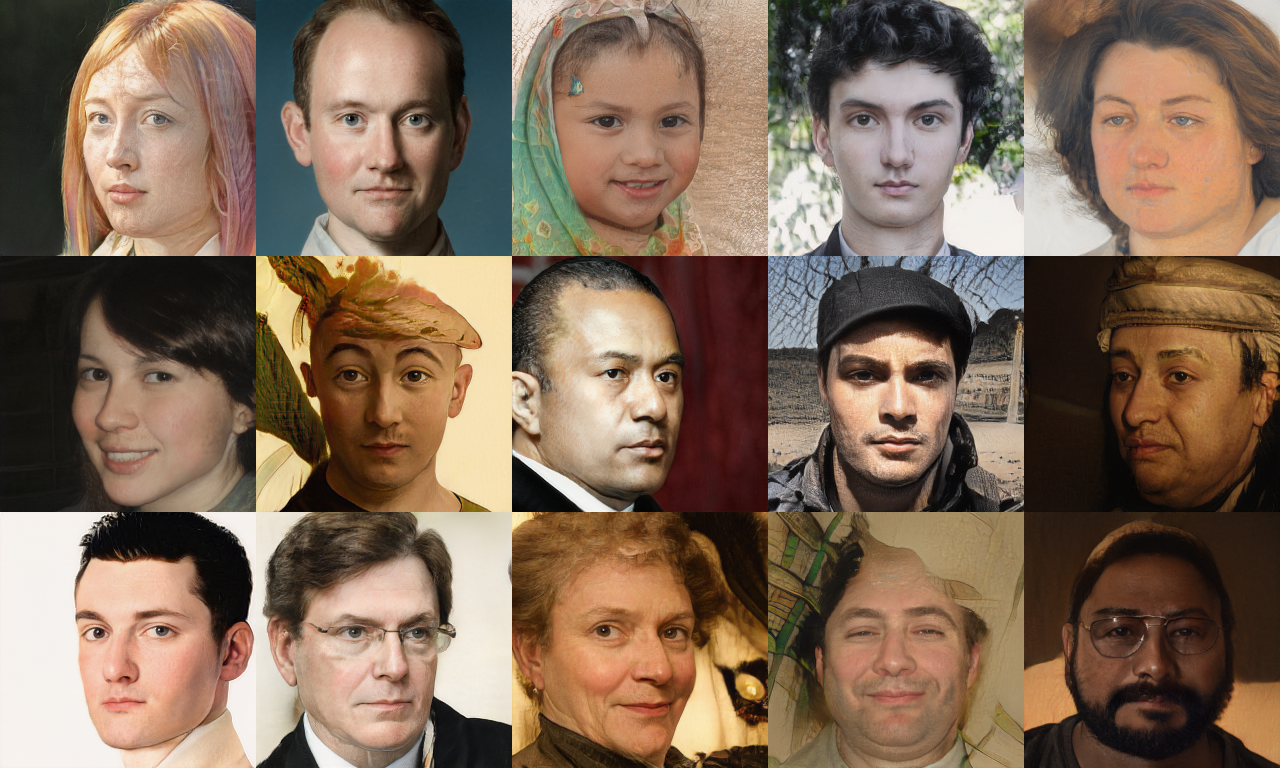
\includegraphics[width=0.8\columnwidth]{./images/picked_images/stylegan2_step_20_full_dataset.png}
		\caption{kimg 20 step of the StyleGAN2 model fine-tuned on the whole MetFaces dataset.}
		\label{fig:figure11}
	\end{center}
\end{figure}
%(stylegan2_step_20_full_dataset.png)[kimg 20 step of the StyleGAN2 model finetuned to the full MetFaces dataset]

\begin{figure}[!h]
	\begin{center}
		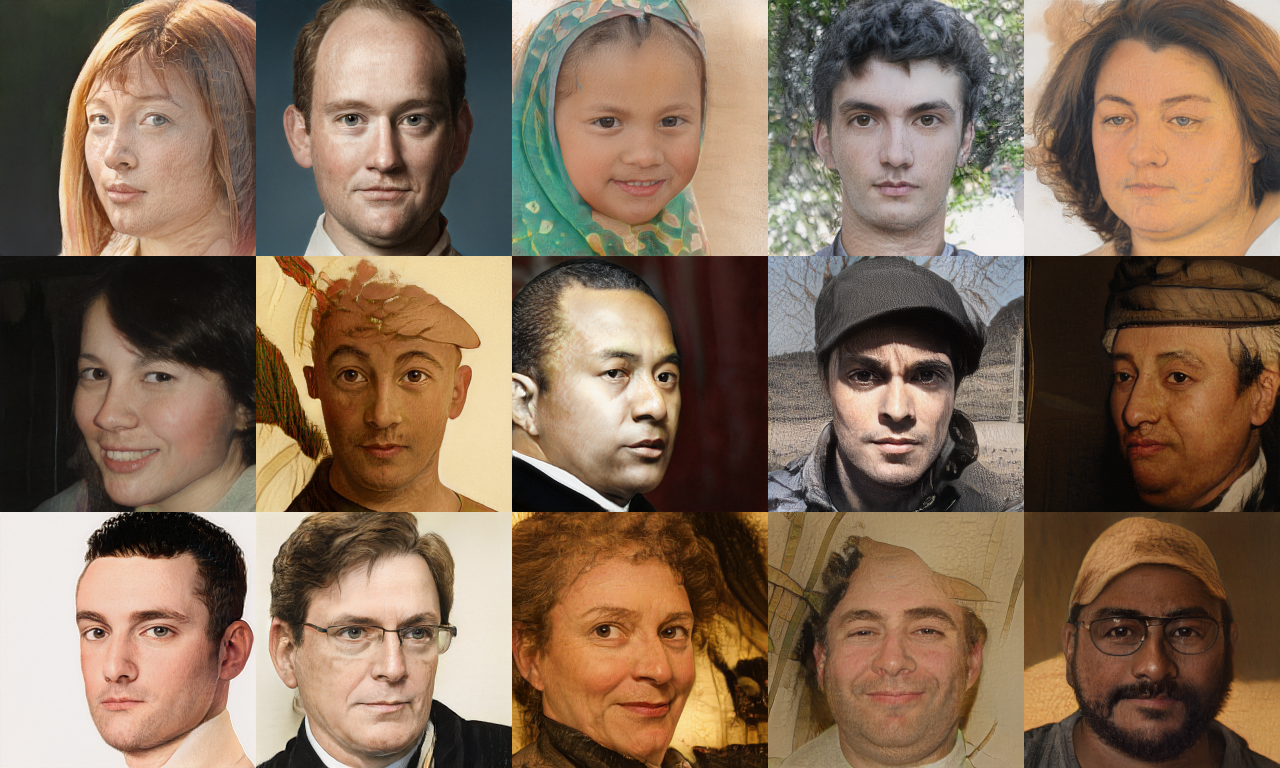
\includegraphics[width=0.8\columnwidth]{./images/picked_images/stylegan2_ADA_step_20_subset100_dataset.png}
		\caption{kimg 20 step of the StyleGAN2-ADA model fine-tuned on 100 MetFaces.}
		\label{fig:figure12}
	\end{center}
\end{figure}
%(stylegan2_ADA_step_20_subset100_dataset.png)[kimg 20 step of the StyleGAN2-ADA model finetuned to 100 MetFaces]

\begin{figure}[!h]
	\begin{center}
		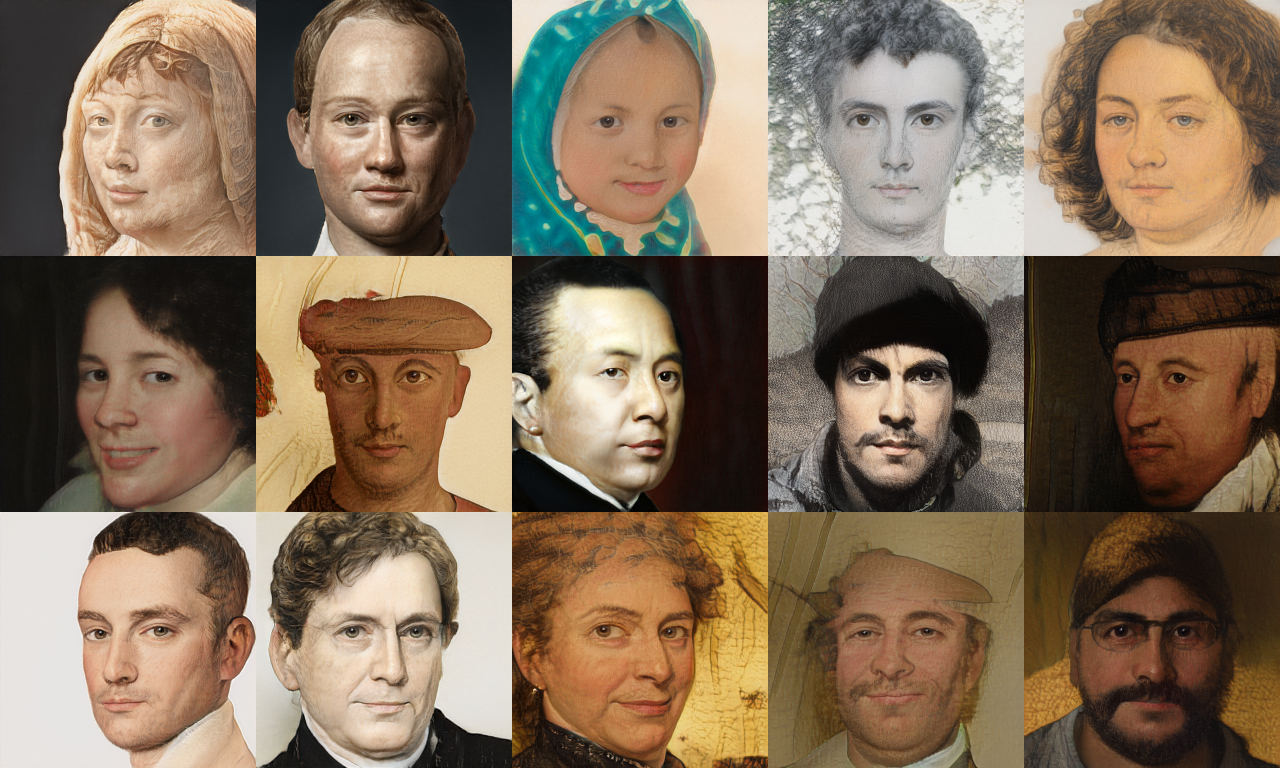
\includegraphics[width=0.8\columnwidth]{./images/picked_images/stylegan2_ADA_step_40_subset100_dataset.png}
		\caption{kimg 40 step of the StyleGAN2-ADA model fine-tuned on 100 MetFaces.}
		\label{fig:figure13}
	\end{center}
\end{figure}
%(stylegan2_ADA_step_40_subset100_dataset.png)[kimg 40 step of the StyleGAN2-ADA model finetuned to 100 MetFaces]


\begin{figure}[!h]
	\begin{center}
		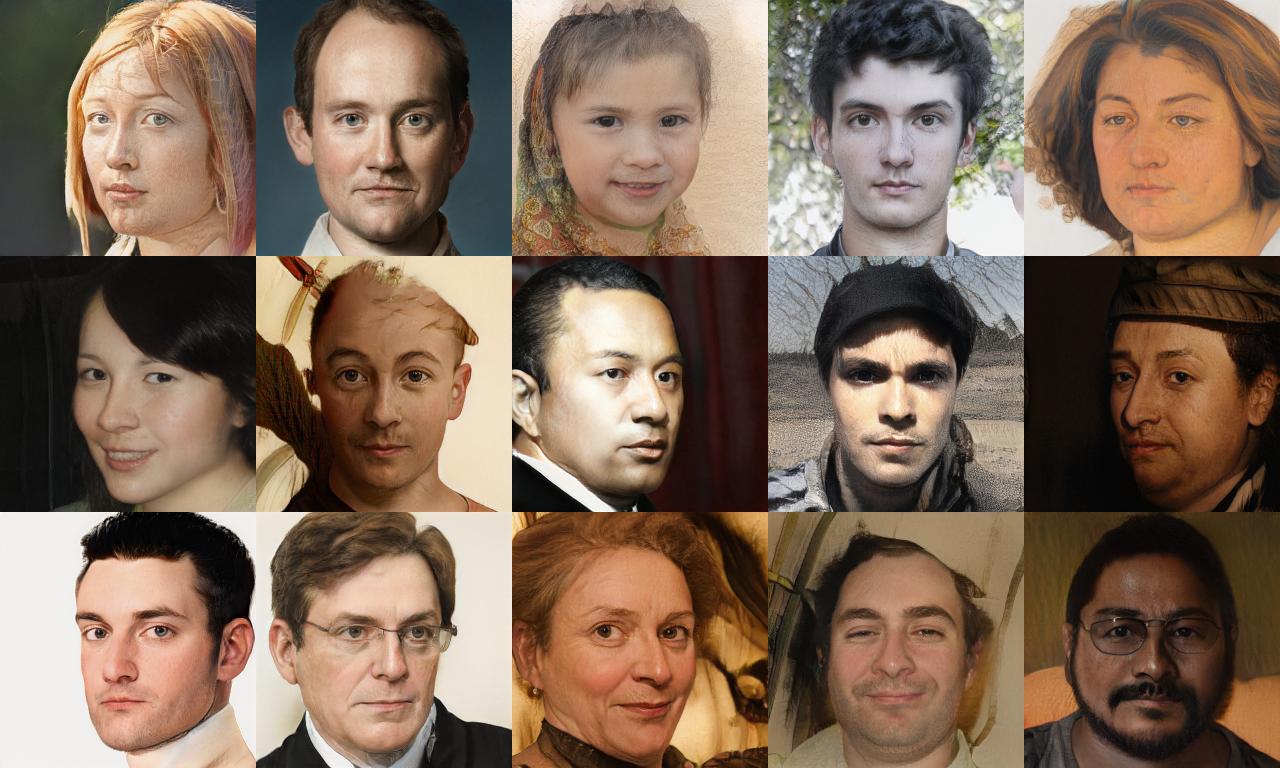
\includegraphics[width=0.8\columnwidth]{./images/picked_images/stylegan2_step_20_subset100_dataset.png}
		\caption{kimg 20 step of the StyleGAN2 model fine-tuned on 100 MetFaces.}
		\label{fig:figure14}
	\end{center}
\end{figure}
%(stylegan2_step_20_subset100_dataset.png)[kimg 20 step of the StyleGAN2 model finetuned to 100 MetFaces]

\begin{figure}[!h]
	\begin{center}
		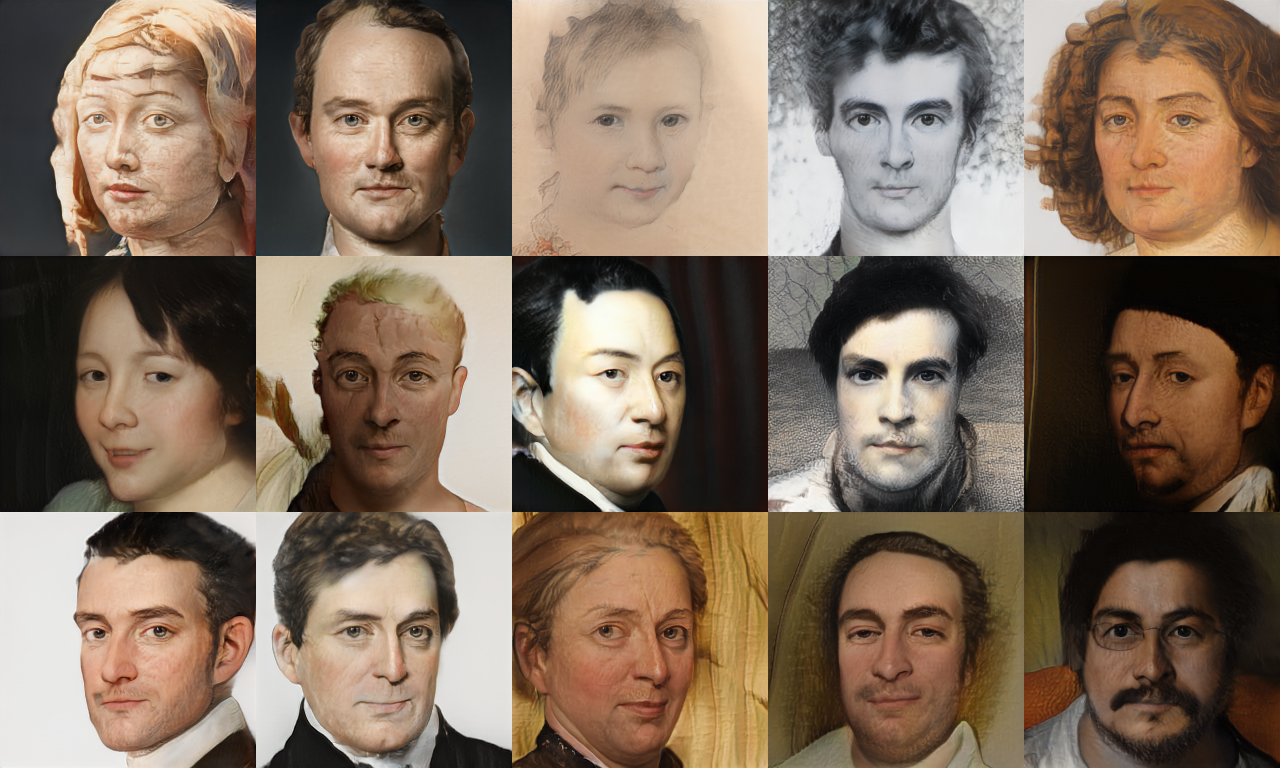
\includegraphics[width=0.8\columnwidth]{./images/picked_images/stylegan2_step_40_subset100_dataset.png}
		\caption{kimg 40 step of the StyleGAN2 model fine-tuned to 100 MetFaces.}
		\label{fig:figure15}
	\end{center}
\end{figure}
%(stylegan2_step_40_subset100_dataset.png)[kimg 40 step of the StyleGAN2 model finetuned to 100 MetFaces]

\end{document}
